
\begin{tcolorbox}
  This is a reminder that, unless differently specified, when we write manifold, chart, atlas, etc. we always mean smooth manifold with (possibly empty) boundary, smooth chart, smooth atlas, etc.
\end{tcolorbox}

\section{Let the fun begin!}
\newthought{It now remains to define derivatives} of functions between smooth manifolds.
And, since we saw that euclidean spaces are manifolds, we must make sure that our definition coincides with the usual one in euclidean spaces.

\begin{marginfigure}[7em]
  \includegraphics{2_1-embedded-sphere-tangent.pdf}
  \label{fig:tan-embedded-sphere}
  \caption{Tangent space to a point of a sphere $\bS^2$ embedded into the ambient space $\R^3$.}
\end{marginfigure}
At the beginning of the previous chapter, we recalled that total derivatives are linear operators.
Since topological spaces are not necessarily vector spaces, then, we need to devise some sort of assignment of vector spaces to points on the manifold.
In this chapter we will see exactly how to do that: we will describe how to associate to each point $p\in M$ on an $n$-dimensional smooth manifold $M$ an $n$-dimensional vector space $T_p M$ called \emph{tangent space to $M$ at $p$}.
For a manifold embedded into an euclidean ambient space this tangent space will coincide with the intuitive understanding of a tangent hyperplane to the point on the manifold, see also Figure~\ref{fig:tan-embedded-sphere}, however it will take a couple of chapters before we can show that it is the case.

As we will see, there are various different definitions of tangent space but, in the end, they all turn out to be equivalent.
Due to a certain amount of freedom in terms of different ``perspectives'' leading to different but equivalent definitions, there is no unique way of introducing tangent spaces.
Just to give you an idea, all the following ideas lead to equivalent definitions (see also~\cite{book:lee}):
\marginnote{Bear in mind that this is not the whole story. For example, it is also possible to ``flip'' the whole construction around, defining first the so-called differentials and with them the cotangent spaces. One can then use these to introduce the tangent spaces.
  This is the approach taken by~\cite{lectures:hitchin} and it is at least worth a look if you want to see a different perspective.}
\begin{itemize}
  \item equivalence classes of curves through a point;
  \item transformation laws of the components of vectors with respect to different charts;
  \item generalization of linear approximation into the idea of an abstract derivation;
  \item derivations in the category of germs of functions.
\end{itemize}

In this course we will start by describing derivations on the space of germs, the approach which emphasizes the local nature of derivations to its extreme.
The equivalence between our approach and the one based on charts will be left as homework, while we will look into the equivalence of velocity vectors of curves and derivations together.

\section{Directional derivatives in euclidean spaces}\label{sec:dd}

Let's take a brief detour.
Suppose that $f: U\subset\R^n\to\R^k$ is a smooth map defined on an open subset $U\subset \R^n$.
In multivariable calculus you have seen that if $x\in U$ and $v\in\R^n$, then the vector $Df(x) v$ can be interpreted as the directional derivative\footnote{Sometimes denoted $D_v f(x)$ instead.} of $f$:
\begin{equation}
  Df(x) v = \lim_{t\to0}\frac{f(x+tv) - f(x)}{t}.
\end{equation}
Then, the partial derivative is obtained as the particular case
\begin{equation}
  \frac{\partial f}{\partial x^j}(x) := D_jf(x) := Df(x) e_j = \lim_{t\to0} \frac{f(x+te_j) - f(x)}{t}.
\end{equation}
Since $f=(f^1, \ldots, f^k)$ takes values in $\R^k$, instead of taking its total derivative $Df$ as above, we can also think to the derivatives of its components.
In this case we can use the standard euclidean coordinates\footnote{See Notation~\ref{ntn:coords}.} $r^1, \ldots, r^n$ to isolate the components and then derive them, that is, we would be deriving $r^i \circ f : \R^n \to \R$.

\newthought{Let's take it slow}, and compare all these various derivatives to each other.
For $f:U\subset\R^n\to\R^k$ and $x\in U$, we have
\begin{marginfigure}[3.5cm]
  \includegraphics{2_3-ederivs.pdf}
\end{marginfigure}
\begin{itemize}
  \item $Df(x)$, the Jacobian matrix, which is a $k\times n$ matrix;
  \item $D_j f(x)$, the $j$-th column of the matrix $Df(x)$, which is an element of $\R^k$ whose components are the derivatives of the components of $f$ with respect to the $j$th coordinate;
  \item $D(r^i\circ f)(x)$, a linear function from $\R^n \to \R$ corresponding to the gradient of the $i$th component of $f$, and which one can see as the $i$th row of the matrix $Df(x)$;
  \item $D_j(r^i\circ f)(x) = \frac{\partial f^i}{\partial x^j}(x)$, a number in $\R$, which corresponds to the $(i,j)$th element $(Df(x))_j^i$ of the matrix $Df(x)$.
\end{itemize}

This notation using $D$ instead of spelling out the partial derivatives, comes with an important advantage.
Let's use it to rewrite the chain rule from Proposition~\ref{thm:chainrule}(\ref{thm:chainrule2}):
\marginnote[1em]{Using Einstein notation, since $l$ is the only index that appears both in lower and upper position, $D_j(r^i\circ g \circ f) (x) = D_l(r^i\circ g)(f(x))\; D_j(r^l \circ f)(x)$.}
\begin{equation}
  D_j(r^i\circ g \circ f) (x) = \sum_{l=1}^k D_l(r^i\circ g)(f(x))\; D_j(r^l \circ f)(x),
\end{equation}
where $1\leq i\leq m, 1\leq j \leq n$.
As you can see, we do not need to explicitly spell out the derivatives in local coordinates on $\R^n$ or $\R^k$ in this new formula.
This will prove extremely convenient for the development of the theory.

\begin{exercise}
  This may look very abstract right now.
  Define some nontrivial function $f: \R^3 \to \R^4$ and compute the 4 objects described above for that function.
\end{exercise}

\section{Germs and derivations}

\newthought{To reach our goal, defining derivations on manifolds}, a direct extension of partial derivatives is not enough: we will need to introduce some more levels of abstraction.

\begin{definition}
  Let $M$ be a smooth manifold and $p\in M$.
  Let $U,V\subset M$ be two neighbourhoods of $p$.
  We say that two functions $f\in C^\infty(U)$ and $g\in C^\infty(V)$ have the same \emph{germ} at $p$ if there exists a neighbourhood $W\subset U\cap V$ of $p$ such that $f|_W \equiv g|_W$.
\end{definition}
\begin{marginfigure}
  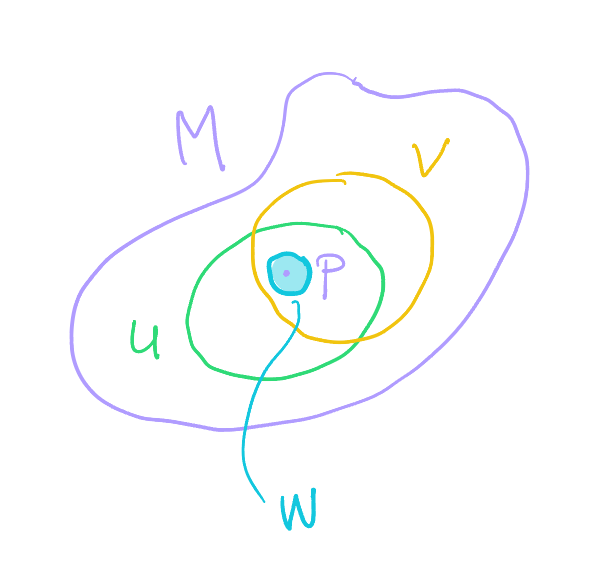
\includegraphics{images/2_3-def_2_3_1.png}
\end{marginfigure}

\begin{exercise}
  Make a drawing to clarify the meaning of this definition.
  Try to define three different functions with the same germ at some point $p$ and with different germs at some other point $p'$.
  Make it concrete: pick $M=\R$ first and then try with $M=\R^3$, and choose some specific values for $p$ and $p'$.
\end{exercise}

Germs define an equivalence relation on the set of smooth functions defined on a neighbourhood of a point $p$: $(U, f) \sim_p (V, g)$ if they have the same germ at $p$. Then, a germ $[f]_p$, where $(U, f)$ is one representative for $[f]_p$, is an equivalence class in the quotient space
\begin{equation}
  C_p^\infty(M) := C^\infty(M)/\!\sim_p.
\end{equation}

\begin{exercise}
  Show that $\sim_p$ defined above is an equivalence relation in $C^\infty(M)$.
\end{exercise}

For $c\in\R$ and $[f]_p, [g]_p$ germs with representatives $(U, f), (V, g)$, we have
\begin{itemize}
  \item $[f]_p + [g]_p$ is the germ with representative $(U\cap V, f+g)$;
  \item $[f]_p [g]_p$ is the germ with representative $(U\cap V, f g)$;
  \item $c[f]_p$ is the germ with representative $(U, cf)$.
\end{itemize}
Therefore, $C_p^\infty(M)$ is also an algebra over $\R$.

\begin{exercise}
  Check that the operations above are well--defined.
\end{exercise}

Germs are the apotheosis of locality: a germ at $p$ has a well--defined value at $p$ and nowhere else.
This results in a map,
\begin{equation}
  \eval_p: C_p^\infty(M) \to \R, \quad
  \eval_p([f]_p) := f(p),
\end{equation}
where $(V,f)$ is any representative of $[f]_p$.
\begin{exercise}
  Check that the $\eval_p$ map is well--defined.
\end{exercise}

We can now go back to our discussion of euclidean derivations to motivate our definition of tangent vectors.

\begin{example}\label{ex:euclideanD}
  Let $U\subset\R^n$ open\footnote{In what follows, we will think of $U$ as both an open subset of $\R^n$ and a smooth manifold depending on what is most convenient for us.} and $f\in C^\infty(U)$.
  For $x\in U$ and $v\in\R^n$ we have seen that $Df(x)$ can be interpreted as a matrix that consumes the vector $v$ to produce a number $Df(x)v$.
  In such interpretation $f$ is fixed and only $x$ and $v$ vary, however there is no reason for this restriction.

  Indeed, an alternative interpretation lets also $f$ vary and considers the action of differentiation as a map
  \begin{equation}
    U \times \R^n \times C^\infty(U) \to \R,\quad
    (x,v,f) \mapsto Df(x) v.
  \end{equation}
  And since we are here changing the cards on the table, let us consider $x$ and $v$ fixed and instead only let $f$ vary:
  \begin{equation}\label{eq:mapxvtoD}
    (x,v):C^\infty(U) \to\R, \quad (x,v)(f) := Df(x)v.
  \end{equation}
  By the definition~\eqref{eq:diff} of the euclidean differential, we know that it is a local concept: the value $Df(x)$ only depends on the value of $f$ in an arbitrarily small neighbourhood of $x$, that is, on the germ of $f$ at $x$.
  Thus we can rephrase~\eqref{eq:mapxvtoD} by saying that $v$ defines a \emph{linear} map
  \begin{equation}
    v : C_x^\infty(U) \to \R, \quad
    v([f]_x) := Df(x) v.
  \end{equation}
  In fact, this is not just a linear map, it also satisfies a \emph{derivation} property, in the sense that
  \begin{equation}
    v([f]_x [g]_x) =
    \eval_x([f]_x)v([g]_x)
    + \eval_x([g]_x)v([f]_x).
  \end{equation}
  Which, rewritten in a more familiar form, is just a way to rewrite the \emph{Leibniz rule}:
  \begin{equation}
    D(fg)(x) v = f(x)\,Dg(x)v + g(x)\,Df(x)v.
  \end{equation}

  Note that we have now \emph{two} different interpretations for $v$: it is both a vector in $\R^n$ and a linear map $C_x^\infty(U) \to \R$ satisfying the derivation property.
\end{example}

Motivated by Example~\ref{ex:euclideanD}, we define a tangent vector as a derivation on the space of germs.

\begin{definition}
  Let $M$ be a smooth manifold of dimension $n$ and let $p\in M$.
  A \emph{tangent vector at $p$} is a linear map
  \marginnote{Keep always in mind that the value $v([f]_p)$ only depends on the value of $f$ around the point $p$.}
  \begin{equation}\label{def:tangentvector}
    v: C_p^\infty(M)\to\R
  \end{equation}
  which is also a derivation, i.e.
  \begin{equation}
    v([f]_p [g]_p) =
    \eval_p([f]_p)v([g]_p)
    + \eval_p([g]_p)v([f]_p).
  \end{equation}

  Since a tangent vector is a linear map from the vector space $C_p^\infty(M)$ to $\R$, the set of all tangent vectors at a point $p$ is itself a vector space\footnote{Exercise: why is this true?} which we denote $T_p M$ and call \emph{tangent space}.
\end{definition}

Let's poke our definition and see if it makes any sense.
Do these vectors at least satisfy the most elementary properties of derivations?
For example, is the derivative of constant functions actually zero?

\begin{lemma}\label{lem:f'0is0forconst}
  Let $M$ be a smooth manifold, let $U\subset M$ be an open set containing $p$ and let $v\in T_p M$.
  Denote by $[c]_p$ the germ of a constant function $(U, p \mapsto c)$.
  Then $v([c]_p) = 0$.
\end{lemma}
\begin{proof}
  Since $[c]_p = c [1]_p$, by linearity we have $v([c]_p) = c v([1]_p)$.
  Thus, it will be enough to show that $v([1]_p) = 0$.
  Since $v$ is a derivation, the algebraic properties of the space of germs imply
  \marginnote{Keep this simple trick in mind, it will be useful in the future.}
  \begin{equation}
    v([1]_p) = v([1]_p [1]_p) = 2 \eval_p([1]_p)v([1]_p) = 2 v([1]_p).
  \end{equation}
  Thus, $v([1]_p) = 0$, concluding the proof.
\end{proof}

As you can see, working with equivalence classes is doable... but it is also unnecessarily cumbersome.
As we did with atlases, we would like to get it over with.

\begin{definition}
  Let $M$ be a smooth manifold and $p\in M$.
  Let $W\subseteq M$ be any neighbourhood of $p$.
  \marginnote{We are still talking about derivations of functions at specific points, not to be confused with the derivations of the algebra $C^\infty(W)$ which we will introduce later and will be maps of the kind $C^\infty(W)\to C^\infty(W)$.}
  A map $w_p:C^\infty(W)\to\R$ is called a \emph{derivation of $C^\infty(W)$ at $p$} if it is linear over $\R$ and satisfies Leibniz rule
  \begin{equation}
    w_p(fg) = f(p)w_p(g) + g(p)w_p(f).
  \end{equation}
\end{definition}

If $v\in T_p M$, then we already saw that $v$ naturally defines a derivation $w_p$ of $C^\infty(W)$ at $p$ for any open neighbourhood $W$ of $p$.
In this case
\begin{equation}\label{eq:derivfromtg}
  w_p(f) := v([f]_p).
\end{equation}
Showing that the opposite is also true will require a bit of work.

\begin{proposition}
  Let $M$ be a smooth manifold, $p\in M$ and $W$ any neighbourhood of $p$.
  Then there is a linear isomorphism between $T_p M$ and the space of derivations of $C^\infty(W)$ at $p$.
\end{proposition}
\begin{proof}
  To prove the theorem we need to invert~\eqref{eq:derivfromtg} and define a tangent vector in terms of of a derivation of $C^\infty(W)$ at $p$.
  We will proceed in three steps.

  \newthought{Step I}. Let $w_p:C^\infty(W) \to\R$ be a derivation at $p$ and suppose that $f\in C^\infty(W)$ is identically zero on a neighbourhood $W_0\subset W$ of $p$.
  We are going to show that $w_p(f)=0$.

  By Proposition~\ref{prop:cutoff}, we can find a cutoff function $\rho:M\to\R$ such that $\rho(p)=1$ in a closed set $W_1 \subset W_0$ and $\supp(\rho) \subset W_0$. Consider now $g = \rho f : W \to \R$.
  Then $g$ is identically zero everywhere in $W$, and thus\footnote{Follows by linearity, exactly as in Lemma~\ref{lem:f'0is0forconst}} $w_p(g) = 0$.
  Using Leibniz rule, the fact that $\rho(p)=1$ and $f(p) = 0$, we get
  \begin{equation}
    0 = w_p(g) = w_p(\rho f) = \rho(p) w_p(f) + f(p)w_p(\rho) = w_p(f).
  \end{equation}

  \newthought{Step II}.
  Let $[f]_p\in C_p^\infty(M)$.
  We want to show that it is always possible to find a representative for $[f]_p$ with domain $W$, that is, there exists $g\in C^\infty(W)$ such that $[g]_p = [f]_p$.
  Let $(V, f)$ be any representative of $[f]_p$.
  Since germs are local, if necessary, we can shrink $V$ so that $V\subset W$.
  Here comes the tricky bit: we need to extend $f$ to a function $g$ defined on $W$ which coincides with $f$ in some neighbourhood of $p$!
  To this end, choose\footnote{We can do this because topological manifolds are locally compact Hausdorff spaces, which implies that every point has a neighbourhood with compact closure. You can take it for granted or have a look at e.g.~\cite[Lemma 4.65]{book:lee:topology} or~\cite{book:munkres:topology}.} a smaller neighbourhood $U$ of $p$ such that $\overline{U}\subset V\subset W$.
  Again, Proposition~\ref{prop:cutoff} comes to the rescue. Apply it with $K=\overline{U}$ and ``$U$'' equal\footnote{Meaning the set that we called $U$ in Proposition~\ref{prop:cutoff} is what we denoted $V$ here.} to $V$, and consider the smooth\footnote{Can you see why it is smooth?} map
  \begin{equation}
    g:W\to\R, \quad
    g(q) := \begin{cases}
      \rho(q)f(q), & q\in V,             \\
      0,           & q \in W\setminus V.
    \end{cases}
  \end{equation}
  Since $g|_U = f$, we have $[g]_p = [f]_p$, proving the claim.

  \newthought{Step III}. We can now complete the proof.
  Let $w_p:C^\infty(W) \to\R$ be a derivation at $p$.
  A tangent vector is a linear map $v:C_p^\infty(M)\to\R$, see~\eqref{def:tangentvector}, and a derivation.
  We would like to define one in terms of $w$.
Given any $[f]_p\in C_p^\infty(W)$, the previous step guarantees that there exists a representative\footnote{Here we have been using $\widetilde{f}$ to emphasize that the specific function may be different from $f$ on the set. Since it makes no difference for any practical purpose, later on we will reuse the same symbol $f$ without further comments.} $(W,\widetilde{f})$ for it, so we can define
  \begin{equation}
    v([f]_p) := w_p(\widetilde{f}), \quad\mbox{where $(W,\widetilde{f})$ is any representative of $[f]_p$}.
  \end{equation}
  Such $v$ is a derivation by construction, so if it is well-defined, we are done.
  To this end, assume that there exists a different representative $(W, g)$ for $[f]_p$.
  Then, by definition, there exists a neighbourhood $V\subset W$ of $p$ such that $\widetilde{f}|_V = g|_V$.
  By linearity, $w_p(\widetilde{f}) - w_p(g) = w_p(\widetilde{f}-g)$ and, by the first step in the proof, $w_p(\widetilde{f}-g) = 0$.

  The assignment $w_p\mapsto v$ inverts~\eqref{eq:derivfromtg}, completing the proof.
\end{proof}

This seemingly innocent proposition, has some very important consequences.

First of all, from now on we are free to interpret tangent vectors in $T_p M$ as derivations of $C^\infty(W)$ at $p$ for \emph{any}\footnote{In particular, it is often convenient to have $W$ coincide with the domain of a chart or with the whole manifold $M$.} open set $W\subseteq M$ containing $p$.
As it turns out, this allows us to give our first example of tangent vector.

\begin{example}\label{ex:partialderivative}
  Let $M$ be a smooth manifold of dimension $n$ and $\varphi: U \to V\subset\R^n$ a chart on $U\subset M$.
  Let $x^i = r^i \circ \varphi$ denote the local coordinates\footnote{See Notation~\ref{ntn:coords}.} of $\varphi$.
  For any $p\in U$, we can define a derivation of $C^\infty(U)$ at $p$ as
  \begin{align}
     & \frac{\partial}{\partial x^i}\Big|_p : C^\infty(U) \to \R,                                                             \\
     & \frac{\partial}{\partial x^i}\Big|_p (f) := \frac{\partial f}{\partial x^i}(p) := D_i(f\circ\varphi^{-1})(\varphi(p)).
  \end{align}
  From now on, it will get more and more convenient to draw commutative diagrams to see ``how things are moving around'':
  \begin{equation}
    \begin{tikzcd}[column sep = huge, row sep = huge]
      M\supset U \arrow[r, "\varphi" description] \arrow[d, "f" description] & V \subset\R^n \arrow [dl, "f\circ\varphi^{-1}" description]\\
      \R &
    \end{tikzcd}
  \end{equation}
  We will soon see that $\left\{\frac{\partial}{\partial x^i}\Big|_p \mid 1\leq i\leq n\right\}$ forms a basis for $T_p M$.
\end{example}

Secondly, we can immediately state some very useful corollaries.

\begin{corollary}\label{cor:tgsubspace}
  Let $M$ be a smooth manifold and let $W\subseteq M$ be a non-empty open set considered as a smooth manifold\footnote{Cf. Exercise~\ref{exe:subsetsmanifolds}.}.
  Then, for any $p\in W$ there is a canonical identification $T_p W \simeq T_p M$.
\end{corollary}

\begin{corollary}\label{cor:derzero}
  Let $M$ be a smooth manifold and $p\in M$.
  Let $W\subseteq M$ be an open neighbourhood of $p$.
  If $f\in C^\infty(W)$ is constant in a neighbourhood of $p$, then $v(f) = 0$ for all $v\in T_p M$.
\end{corollary}

With these new tools at hand, we are ready to state and prove an important result on the size of the tangent spaces.
As it turns out, if $M$ is an $n$-dimensional manifold, $T_pM$ is a finite dimensional vector space of the same dimension $n$, and thus isomorphic to $\R^n$.

\begin{theorem}\label{thm:dimensionTpM}
  Let $M$ be a smooth manifold of dimension $n$ and $p\in M$.
  Then $T_pM$ is a vector space of dimension $n$.
\end{theorem}

The theorem will follow immediately once we construct a basis for $T_pM$.
To that end, we need a preliminary result from multivariable analysis.

\begin{lemma}\label{lem:Taylor}
  Let $U\subset\R^n$, $0\in U$, be a star-shaped\footnote{An open set $U\subset\R^n$ containing the origin, $0\in U$, is called \emph{star-shaped} if $U$ also contains the line segment from $0$ to $x$ for any $x\in U$.} open set and $h\in C^\infty(U)$.
  Then, there exist $n$ smooth functions $g_i: U \to \R$, $1\leq i \leq n$, such that $g_i(0) = D_i h(0)$ and
  \begin{equation}
    h = h(0) + r^i g_i
  \end{equation}
  \marginnote[-2em]{$\leftarrow$ This is our first use of Einstein notation, this equation should be read as $h(x) = h(0) + \sum_{i=1}^n r^i(x) g_i(x)$.
    Using the global euclidean chart, $x^i = r^i(x)$ and $h(x) = h(0) + \sum_{i=1}^n x^i g_i(x)$, which you may recognize as the first iteration of the usual Taylor-MacLaurin formula.}
  where $r^i$ are the coordinates introduced in Notation~\ref{ntn:coords}.
\end{lemma}
\begin{proof}
  Fix a point $x = (x^1, \ldots, x^n) \in U$.
  Let $\gamma_x:[0,1]\to U$ denote the line segment from $0$ to $x$, parametrized as $\gamma_x(t) = tx$.

  By the chain rule,
  \begin{equation}
    \frac{d}{dt}(h \circ \gamma_x) (t) = \left(D_i h(t x)\right) \cdot \frac{d}{dt} (t x^i) = x^i D_i h(t x).
  \end{equation}
  \marginnote[-2.5em]{$\leftarrow$ Again, due to Einstein notation, the right hand side should be read as $\sum_{i=1}^n x^i D_i h(t x)$.}
  The fundamental theorem of calculus then implies
  \begin{align}
    h(x) - h(0) & = (h \circ \gamma_x)(1) - (h \circ \gamma_x)(0)                                 \\
                & = \int_0^1 \frac{d}{dt}(h \circ \gamma_x)(t)\;dt = x^i \int_0^1 D_i h(tx)\; dt.
  \end{align}
  \marginnote[-2.3em]{$\leftarrow$ For one last time, due to Einstein notation, the right hand side should be read as $\sum_{i=1}^n x^i \int_0^1 D_i h(t x)\; dt$.}

  Since $x^i = r^i(x)$ by definition, the theorem follows by defining
  \begin{equation}
    g_i(x) := \int_0^1 D_i h(tx)\; dt.
  \end{equation}
\end{proof}

Theorem~\ref{thm:dimensionTpM} now follows from the next statement.

\begin{proposition}\label{prop:basis_TpM}
  Let $M$ be a smooth manifold of dimension $n$ and $p\in M$.
  Let $\varphi: U \to V$ be a chart on $M$ around $p$, i.e. $p\in U$.
  Then any tangent vector $v\in T_p M$ can be uniquely written as a linear combination
  \begin{equation}
    v = v^i \frac{\partial}{\partial x^i}\Big|_p, \quad v_i = v(x^i).
  \end{equation}
  \marginnote[-3em]{$\leftarrow$ Since we consider upper indices in the denominator as lower indices, the equation should be read as $v = \sum_{i=1}^n v^i \frac{\partial}{\partial x^i}\Big|_p$. If $M=\R^n$, what we are saying here is that $v(f) = v\cdot\nabla f = Df\; v$, that is, $v$ acts as the directional derivative in its direction.}
  Thus, $\left\{\frac{\partial}{\partial x^i}\Big|_p\;\mid\; 1\leq i\leq n\right\}$ is a basis of $T_p M$.
\end{proposition}
\begin{proof}
  We may assume without loss of generality that $\varphi(p) = 0$ and, thanks to Corollary~\ref{cor:tgsubspace}, that $U$ is star-shaped.
  Let $f\in C^\infty(U)$.
  By Lemma~\ref{lem:Taylor} with $h = f \circ \varphi^{-1}$ we get
  \begin{equation}
    f = f(p) + x^i (g_i \circ \varphi),
    \quad g_i(0) = D_i (f \circ \varphi^{-1})(0) = \frac{\partial}{\partial x_i}\Big|_p(f).
  \end{equation}
  \marginnote{If we are careful with the meaning of our notation, we could write more succintly $\frac{\partial f}{\partial x_i}(p)$ in place of $\frac{\partial}{\partial x_i}\big|_p(f)$ in the same fashion as in Example~\ref{ex:partialderivative}.}
  Thus, for any derivation $v$, we obtain
  \begin{equation}
    v(f) = v(f(p)) + v(x^i)g_i(0) + x^i(p) v(g_i\circ\varphi) = v(x^i)  \frac{\partial}{\partial x_i}\Big|_p(f).
  \end{equation}
  The right hand side is obtained observing that $\varphi(p) = 0$, and thus the components $x^i(p) = 0$ are all zero, and applying Corollary~\ref{cor:derzero} to the constant $f(p)$, which implies $v(f(p)) = 0$.

  It follows that the set $\left\{\frac{\partial}{\partial x^i}\Big|_p\;\mid\; 1\leq i\leq n\right\}$ spans $T_p M$.
  We now need to show that its elements are linearly independent.
  Observe that
  \begin{align}
    \frac{\partial}{\partial x_i}\Big|_p (x^j) & =
    \frac{\partial}{\partial x_i}\Big|_p (r^j \circ \varphi)                                               \\
                                               & = D_i (r^j \circ \varphi \circ \varphi^{-1}) (\varphi(p)) \\
                                               & = D_i r^j(\varphi(p)) = \delta^j_i.
  \end{align}
  Thus, if
  \begin{equation}
    v = a^i \frac{\partial}{\partial x_i}\Big|_p = 0,
  \end{equation}
  by letting $v$ act on $x^j$, $1\leq j\leq n$, we obtain $(a^1, \ldots, a^n) = 0$, proving the linear independence.
\end{proof}

\begin{remark}[Change of coordinates]\label{rmk:chg_coords}
  Suppose $\varphi$ and $\psi$ are two different charts about $p$, with corresponding coordinates $x^i := r^i \circ \varphi$ and $y^i := r^i \circ \psi$.
  Taking $v = \frac{\partial}{\partial y^j}\Big|_p$ in the previous proposition implies that
  \begin{equation}
    \frac{\partial}{\partial y^j}\Big|_p =
    \frac{\partial}{\partial y^j}\Big|_p (x^i) \frac{\partial}{\partial x^i}\Big|_p.
  \end{equation}
  \marginnote[-3em]{If we start getting used to thinking of these vectors as actual derivatives and hide the dependence on $p$, then the equation on the left can be rewritten as $\frac{\partial}{\partial y^j} =
      \frac{\partial x^i}{\partial y^j} \frac{\partial}{\partial x^i}$.}
  %
  Expanding the definitions, we get
  \begin{equation}
    \frac{\partial}{\partial y^j}\Big|_p (x^i) =
    D_j(x^i\circ\psi^{-1})(\psi(p)) =
    D_j(r^i \circ \varphi \circ \psi^{-1})(\psi(p)),
  \end{equation}
  which is the $(i,j)$th entry in the matrix $D(\varphi\circ\psi^{-1})(\psi(p))$ as discussed at the beginning of Section~\ref{sec:dd}.
  In other words, $D(\varphi\circ\psi^{-1})(\psi(p))$ is the transition matrix from the basis $\left\{\frac{\partial}{\partial y^i}\Big|_p\;\mid\; 1\leq i\leq n\right\}$ to the basis $\left\{\frac{\partial}{\partial x^i}\Big|_p\;\mid\; 1\leq i\leq n\right\}$.
\end{remark}

\begin{example}
  The transition map between the standard euclidean coordinates and the polar coordinates on appropriate open sets in $\R^2$ is given by $(x,y) = (\rho\cos(\theta), \rho\sin(\theta))$. Let $p\in\R^2$ denote the point with coordinates $(\rho, \theta) = (3, \pi)$ and $v\in T_p\R^2$ the tangent vector with polar coordinate representation
  \begin{equation}
    v = 5\frac{\partial}{\partial \rho}\Big|_p - \frac{\partial}{\partial \theta}\Big|_p.
  \end{equation}
  Applying the equations in Remark~\ref{rmk:chg_coords}, we get
  \begin{align}
    \frac{\partial}{\partial \rho}\Big|_p
     & = \cos(\pi)\frac{\partial}{\partial x}\Big|_p + \sin(\pi)\frac{\partial}{\partial y}\Big|_p = - \frac{\partial}{\partial x}\Big|_p      \\
    \frac{\partial}{\partial \theta}\Big|_p
     & = -3\sin(\pi)\frac{\partial}{\partial x}\Big|_p + 3\cos(\pi)\frac{\partial}{\partial y}\Big|_p = -3 \frac{\partial}{\partial y}\Big|_p,
  \end{align}
  and thus, the vector $v$ in standard coordinates is represented by
  \begin{equation}
    v = - 5 \frac{\partial}{\partial x}\Big|_p + 3 \frac{\partial}{\partial y}\Big|_p.
  \end{equation}
\end{example}

\begin{exercise}
  Let $(x,y)$ denote the standard coordinates on $\R^2$.
  \begin{enumerate}
    \item Show that $(\widetilde{x}, \widetilde{y})$, where
          \begin{equation}
            \widetilde{x} = x
            \quad\mbox{and}\quad
            \widetilde{y} = y + x^3,
          \end{equation}
          are global smooth coordinates in $\R^2$.
    \item Let $p=(1,0)\in\R^2$ in standard coordinates.
          Show that $\frac{\partial}{\partial x}\Big|_p \neq \frac{\partial}{\partial \widetilde x}\Big|_p$ even though the respective coordinate functions are identically equal.
  \end{enumerate}
  This shows that the coordinate vectors in the tangent space depend on the whole coordinate system and not just on the single coordinate function they are associated to.
\end{exercise}

\newthought{We already mentioned} that there are multiple equivalent definitions of the tangent space. In the following exercises you will provide one in terms of charts and euclidean derivatives.
Soon, we will see yet another definition.

\begin{exercise}\label{exe:vsstruct}
  Let $\{V_\alpha \mid \alpha\in A\}$ be a family of vector spaces indexed by a set $A$, let $W$ be a fixed set and let $T_\alpha: V_\alpha\to W$ be a bijection for all $\alpha\in A$.
  Assume that for any $\alpha, \beta \in A$, the composition $T_\beta^{-1}\circ T_\alpha : V_\alpha \to V_\beta$ is a linear isomorphism.
  Show that there is a unique vector space structure on $W$ such that each $T_\alpha$ is a linear isomorphism.
\end{exercise}

\begin{exercise}[Tangent vectors as equivalence classes of charts and vectors]
  Let $M$ be a smooth $m$-manifold with maximal smooth atlas $\cA$.
  For $p\in M$, let $\cA_p \subset \cA$ denote the set of charts $\varphi\in\cA$ such that $p$ lies in the domain of $\varphi$.
  \begin{enumerate}
    \item Show that
          \begin{equation}
            (v,\varphi) \sim (w, \psi)
            \quad\Longleftrightarrow\quad
            D(\psi \circ \varphi^{-1})(\varphi(p))v = w.
          \end{equation}
          defines an equivalence relation on $\R^m\times\cA_p$.
    \item Let $\cT_p$ denote the set of equivalence classes $[(v,\varphi)]\in \R^m\times\cA_p/\!\sim$. For $\varphi\in\cA_p$, show that the map $T_\varphi:\R^m\to\cT_p$ given by $T_\varphi v := [(v,\varphi)]$ is a bijection.
          Deduce\footnote{Hint: use the previous exercise!} that $\cT_p$ admits a unique vector space structure such that each $T_\varphi$ is a linear isomorphism.
    \item Let $\varphi$ be a chart defined on a neighbourhood of $p$ with local coordinates $x^i = r^i \circ \varphi$ and let $\hat T_\varphi :\R^m \to T_pM$ denote\footnote{As it turns out, this is the same as $T_x$ defined in~\eqref{def:lin_iso_Tp}, however in this exercise we use a different notation to emphasize the dependence on the chart.} the linear isomorphism defined by $\hat T_\varphi e_i = \frac{\partial}{\partial x^i}\big|_p$.
          Show that there exists a linear isomorphism $\mathcal{S}_p:\cT_p\to T_pM$ which in addition satisfies $\mathcal{S}_p \circ T_\varphi = \hat T_\varphi$ for every chart $\varphi$ about $p$.
  \end{enumerate}
\end{exercise}

\section{The differential of a smooth map}\label{sec:diffsmooth}

\newthought{In the case of a smooth map between euclidean spaces}, the total derivative of the map at a point (represented by its Jacobian matrix) is a linear map that represents the best linear approximation to the map near the given point.
\marginnote{If you are curious about what happens if you consider higher order approximations, try to look up \emph{Jet Space} with your favourite search engine.}
In the manifold case there is a similar linear map but, as we discussed, it makes no sense to talk about a linear map between manifolds: we need to find a suitable linear map between tangent spaces.

It should not come a surprise that with the constructions developed so far not only do we have one such map, but we can directly relate it to a derivative.

\begin{definition}\label{def:differentialMap}
  Let $F: M \to N$ be a smooth map between the smooth manifolds $M$ and $N$, and let $p\in M$.
  The \emph{differential $d F_p$ of $F$ at $p$} is the map\footnote{In the differential geometry literature, the differential has many names: you can find it called \emph{tangent map}, \emph{total derivative} or \emph{derivative} of $F$.
    Since it ``pushes'' tangent vectors forward from the domain manifold to the codomain, it is also called the \emph{pushforward}. If that was not enough, different authors use different notations for it: besides $dF_p(v)$, you can find $F_* v_p$, $F'(p)$, $T_pF$, $DF(p)[v]$ or variations thereof.}
  \begin{equation}
    d F_p : T_p M \to T_{F(p)} N, \qquad d F_p (v) (f) := v(f\circ F), \quad \forall f\in C^\infty(N).
  \end{equation}
\end{definition}

Indeed, $v \mapsto d F_p (v)$ is a linear map (why?) defining a derivation at $F(p)$ acting on functions in $C^\infty(N)$ (why?) and, as such, is also a tangent vector in $T_{F(p)}N$.

\begin{exercise}
  Answer the two \emph{(why?)} above.
\end{exercise}
\begin{exercise}
  Let $M = \R^3$ and $N = \R^2$ with coordinates $x=(x^1,x^2,x^3)$ and $y=(y^1,y^2)$ respectively.
  Consider the function $F(x^1,x^2,x^3) = (x^1 x^3, (x^2)^2-1)$.
  What is $d F_{(1,1,1)} \left(\frac{\partial}{\partial x^1} - 2 \frac{\partial}{\partial x^2}\right)$?
\end{exercise}

\begin{theorem}[The chain rule on manifolds]\label{thm:chainrule_mfld}
  Let $M, N, P$ be smooth manifolds and $F: M \to N$, $G: N\to P$ be two smooth maps. Then
  \marginnote{The alternative $D$ notation, in this case, makes the relation to the usual chain rule even more evident: $D(G\circ F)(p) = DG(F(p))\circ DF(p)$.}
  \begin{equation}
    d(G\circ F)_p = dG_{F(p)} \circ dF_p.
  \end{equation}
\end{theorem}
\begin{proof}
  Since $dF_p : T_p M \to T_{F(p)}N$ and $dG_{F(p)}: T_{F(p)}N \to T_{G(F(p))}P$, the map $d(G\circ F)_p: T_p M \to T_{G(F(p))}P$ has the right domain and codomain.
  Take now $v\in T_p M$ and $f\in C^\infty(P)$. We get
  \begin{align}
    d(G\circ F)_p(v)(f) & = v(f\circ G \circ F)
    = dF_p (v)(f\circ G)                                                  \\
                        & \stackrel{(\bigstar)}{=} dG_{F(p)}(dF_p (v))(f)
    = dG_{F(p)} \circ dF_p (v)(f),
  \end{align}
  where in $(\bigstar)$ we used the fact that $dF_p (v)\in T_{F(p)}N$.
\end{proof}

\begin{remark}
  The differential of the identity map $\id_M:M\to M$ at any point $p\in M$ is the identity map
  \begin{equation}
    \id_{T_pM}: T_pM \to T_pM.
  \end{equation}
  Indeed, $d (\id_M)_p(v)(f) = v(f\circ\id_M) = v(f)$ for any $v\in T_pM$ and any $f\in C^\infty(M)$.
\end{remark}

The definition we gave seems quite abstract, let's see what it looks like in coordinates.

\begin{proposition}\label{prop:DiffCoords}
  Let $F:M^m\to N^n$ be a smooth map between smooth manifolds.
  Let $p\in M$, and let $\varphi : U \to \varphi(U)$ be a chart on $M$ about $p$ and $\psi: V \to \psi(V)$ be a chart on $N$ about $F(p)$.
  If $(x^i)$ denotes the local coordinates of $\varphi$ and $(y^i)$ the ones of $\psi$, the matrix of $dF_p$ with respect to the bases $\left\{\frac{\partial}{\partial x^j}\big|_p \;\mid\; j=1,\ldots,m\right\}$ of $T_pM$ and $\left\{\frac{\partial}{\partial y^j}\big|_{F(p)} \;\mid\; j=1,\ldots,n\right\}$ of $T_{F(p)}N$ is given by the Jacobian matrix $D(\psi\circ F \circ\varphi^{-1})(\varphi(p))$.
\end{proposition}
\begin{proof}
  The proof follows from the following direct computation after observing that the number $D_j(r^i \circ \psi \circ F \circ \varphi^{-1})(\varphi(p))$ is the $(i,j)$ entry of the Jacobian matrix $D(\psi\circ F \circ\varphi^{-1})(\varphi(p))$. For any $j=1,\ldots,m$, Remark~\ref{rmk:chg_coords} implies
  \begin{align}
    dF_p \left(\frac{\partial}{\partial x^j}\Big|_p\right)
     & =                                                                                                   %\sum_{i=1}^n 
    dF_p \left(\frac{\partial}{\partial x^j}\Big|_p\right) (y^i) \frac{\partial}{\partial y^i}\Big|_{F(p)} \\
     & =                                                                                                   %\sum_{i=1}^n 
    \frac{\partial}{\partial x^j}\Big|_p (y^i \circ F) \frac{\partial}{\partial y^i}\Big|_{F(p)}           \\
     & =                                                                                                   %\sum_{i=1}^n 
    D_j(r^i \circ \psi \circ F \circ \varphi^{-1})(\varphi(p)) \frac{\partial}{\partial y^i}\Big|_{F(p)}.
  \end{align}
\end{proof}

\begin{exercise}
  Show that the matrix of $d F_p$ in terms of the coordinate bases is
  \begin{equation}
    \begin{pmatrix}
      \frac{\partial F^1}{\partial x^1} (p) & \cdot  & \frac{\partial F^1}{\partial x^n} (p) \\
      \vdots                                & \ddots & \vdots                                \\
      \frac{\partial F^m}{\partial x^1} (p) & \cdot  & \frac{\partial F^m}{\partial x^n} (p)
    \end{pmatrix}
  \end{equation}
  without using the Proposition above. Here $\frac{\partial F^i}{\partial x^j} (p) = \frac{\partial}{\partial x^j}\big|_p (F^i)$, where $F^i$ is the $i$th component of $F$ with respect to the chart with coordinates $y^j$.\\
  \textit{\small Hint: show that $d F_p \left(\frac{\partial}{\partial x^i}\big|_p\right) (f) = \left(\frac{\partial F^j}{\partial x^i} (p) \frac{\partial}{\partial y^j}\big|_{F(p)}\right) (f)$.}
\end{exercise}

\newthought{A particularly important consequence} of this theorem is that if we set $M=\R^m$ and $N=\R^n$ our definition coincides with the euclidean notion.
This is easily checked by taking $\varphi = \id_{\R^m}$ and $\psi=\id_{\R^n}$.
Then the coordinates $(x^1,\ldots,x^m)$ are the standard euclidean coordinates for $\R^m$ and the coordinates $(y^1,\ldots,y^n)$ the ones for $\R^n$.

Let $f:U\subset\R^m\to\R^n$ be a smooth function and define the linear isomorphisms
\begin{equation}\label{def:lin_iso_Tp}
  \begin{split}
    &T_x : \R^m \to T_x\R^m,\quad T_x e_i = \frac{\partial}{\partial x^i}\Big|_x\\
    &T_y : \R^n \to T_y\R^n,\quad T_y e_i' = \frac{\partial}{\partial y^i}\Big|_y
  \end{split},
\end{equation}
where $\{e_1,\ldots,e_m\}$ denotes the standard basis of $\R^m$ and $\{e_1',\ldots,e_n'\}$ denotes the standard basis of $\R^n$.

On the one hand, we have the total derivative $Df(x):\R^m\to\R^n$ from multivariable calculus: a linear map, the Jacobian matrix of partial derivatives.
On the other, we have the differential $df_x : T_x \R^m \to T_{f(x)}\R^m$ defined above: also a linear map, related to the Jacobian matrix of partial derivatives by Proposition~\ref{prop:DiffCoords}.
In fact we know more, since Proposition~\ref{prop:DiffCoords} tells us that the following diagram commutes:
\begin{equation}
  \begin{tikzcd}[row sep=huge, column sep=huge]
    \R^m \arrow[r, "Df(x)"] \arrow[d, "T_x"]
    & \R^n \arrow[d, "T_{f(x)}"] \\
    T_x\R^m \arrow[r, "df_x"]
    & T_{f(x)}\R^n
  \end{tikzcd}.
\end{equation}

More generally, the same kind of reasoning shows the following fact. For any smooth map $F:M^m \to N^n$ between smooth manifolds, if $\varphi$ is a chart about $x\in M$ with coordinates $(x^i)$ and $\psi$ is a chart about $y=F(x)\in N$ with coordinates $(y^i)$, the following diagram commutes:
\marginnote{Recall that the following commutes: \begin{equation}
    \begin{tikzcd}[row sep=huge, column sep=huge, ampersand replacement=\&]
      M \arrow[r, "F"] \arrow[d, "\varphi"] \& N \arrow[d, "\psi"]\\
      \R^m \arrow[r, "\psi \circ F \circ \varphi^{-1}"]
      \& \R^n
    \end{tikzcd}.
  \end{equation}}
\begin{equation}
  \begin{tikzcd}[row sep=huge, column sep=huge]
    \R^m \arrow[r, "D(\psi \circ F \circ \varphi^{-1})(\varphi(x))"] \arrow[d, "T_x"]
    & \R^n \arrow[d, "T_{F(x)}"] \\
    T_xM \arrow[r, "dF_x"]
    & T_{F(x)}N
  \end{tikzcd},
\end{equation}
where $T_x$ and $T_{F(x)}$ are defined as above.

\newthought{An aspect of the construction above is particularly disturbing}: it forced us to fix a basis on the spaces; if this were truly necessary it would defeat the purpose of this whole chapter.
Fortunately for us, the following exercise shows that, at any given point, the tangent space to a vector space is \emph{canonically}\footnote{That is, independently of the choice of basis.} identified with the vector space itself.

\begin{exercise}\label{ex:tg_curve_iso}
  Let $V$ and $W$ be finite-dimensional vector spaces, endowed with their standard smooth structure (see Exercise~\ref{exe:subsetsmanifolds}).
  \begin{enumerate}
    \item Fix $a\in V$. For any vector $v\in V$ define a map $\cT_a(v) : C^\infty(V) \to \R$ by
          \begin{equation}
            \cT_a(v) f = \frac{d}{dt}\Big|_{t=0} f(a + tv).
          \end{equation}
          Show that the map $v\mapsto \cT_a(v) : V \to T_aV$ is an isomorphism of vector spaces.
    \item Let $L:V\to W$ be a linear map. Show for any $a\in V$ that the following diagram commutes:
          \begin{equation}
            \begin{tikzcd}[row sep=huge, column sep=huge]
              V \arrow[r, "L"] \arrow[d, "\cT_a"]
              & W \arrow[d, "\cT_{La}"] \\
              T_aV \arrow[r, "dL_a"]
              & T_{La}W
            \end{tikzcd}.
          \end{equation}
  \end{enumerate}
\end{exercise}

An important consequence of what we have seen so far is that we can routinely \emph{identify} tangent vectors to a finite-dimensional vector space with elements of the space itself.
More generally, if $M$ is an open submanifold of a vector space $V$, we can combine the identifications $T_p M \simeq T_p V \simeq V$ to obtain a canonical identification of each tangent space to $M$ with $V$.
For example, since $GL_n(\R)$ is an open submanifold of the vector space $\mathrm{Mat}(n, \R)$, we can identify its tangent space at each point $X\in GL_n(\R)$ with the full space of matrices $\mathrm{Mat}(n, \R)$.

\begin{exercise}[Tangent space of a product manifold]
  Let $M_1, \ldots, M_k$ be smooth manifolds (without boundary\footnote{The statement is true also if one (only one!) of the $M_i$ spaces is a smooth manifold with boundary. If there is more than one manifold with boundary, the product space will have ``corners'' that cannot be mapped to half spaces and thus is not a smooth manifold, as a simple example you can consider the closed square $[0,1]\times [0,1]$.}), and for each $j$ let $\pi_j:M_1\times\cdots\times M_k \to M_j$ be the projection onto the $M_j$ factor.
  For any point $p=(p_1,\ldots,p_k)\in M_1\times\cdots\times M_k$, the map
  \begin{align}
    \sigma & : T_p(M_1\times\cdots\times M_k) \to T_p M_1\times\cdots\times T_p M_k \\
    \sigma & : v \mapsto \left(d(\pi_1)_p(v), \ldots, d(\pi_k)_p(v)\right)
  \end{align}
  is an isomorphism.
\end{exercise}

\begin{remark}
  When $M$ is a smooth manifold with boundary and $p$ is an interior point, all the discussions above apply verbatim. In particular, the tangent space at a boundary point of an $n$-dimensional manifold with boundary is also an $n$-dimensional real vector space that can be identified (non-uniquely) with $\R^n$ using a chart containing that point.

  For $p\in\partial M$ the only change that needs to be made is to substitute $\cH^n$ for $\R^n$, with the understanding that the notation $\frac{\partial}{\partial x^i}\big|_{\varphi(p)}$ can be used interchangeably to denote either an element of $T_{\varphi(p)}\R^n$ or of $T_{\varphi(p)}\cH^n$. In the latter case, the $n$th coordinate vector $\frac{\partial}{\partial x^n}\big|_{p}$ should be interpreted as a one-sided derivative.
\end{remark}

In the next section we will give yet another alternative way of defining tangent vectors: less elegant but easier to compute.


\section{Tangent vectors as tangents to curves}

\begin{marginfigure}[1em]
  \includegraphics{2_2-curve-on-M.pdf}
\end{marginfigure}

Exercise~\ref{ex:tg_curve_iso} may have left some thoughts hanging in the air...
From the look of it, it seems that there is a relation between tangent spaces and the velocity of a body moving with constant speed.
In this section we will further explore these thoughts.

\begin{definition}
  If $M$ is a manifold with or without boundary, we define a \emph{(parametrized) curve in M} to be a smooth\footnote{Continuously differentiable would be enough, but assuming it smooth simplifies the exposition.} map $\gamma : I \to M$, where $I=(a,b)\subseteq\R$ is an interval.
  \marginnote{Conventionally, $b=-a=\epsilon>0$ (the reason will be clear in a second) and we denote the coordinate on $\R$ by $t$ and the derivative of $\gamma$ at a point $t$ by $\gamma'(t)$. We say that a curve \emph{starts at $p\in M$} if $0\in I$ and $\gamma(0) = p$.}
\end{definition}

Fix $t\in(a,b)$.
A priori we have two different ways to define the \emph{velocity vector of $\gamma$ at a time $t$}, that is, an element $\gamma'(t) \in T_{\gamma(t)}M$:
\begin{enumerate}[(i)]
  \item We can define a derivation of $C^\infty(M)$ at $\gamma(t)$ by setting
        \begin{equation}\label{eq:tg_curve_der}
          \gamma'(t) (f) := (f\circ\gamma)'(t), \quad f\in C^\infty(M).
        \end{equation}
        \begin{exercise}
          Show that this is indeed a derivation of $C^\infty(M)$ at $\gamma(t)$.
        \end{exercise}
  \item If we think of $\gamma$ as a smooth map between manifolds, we can define the tangent vector via the differential $d\gamma_t$:
        \begin{equation}\label{eq:tg_curve_diff}
          \gamma'(t):= d\gamma_t\left(\frac{\partial}{\partial t}\Big|_t\right) \in T_{\gamma(t)}M.
        \end{equation}
\end{enumerate}

Do these definitions agree?
One way to check is to pick a chart $\varphi: U \to \varphi(U)$ in a neighbourhood of $\gamma(t)$, and compare the expressions in local coordinates. Let $(x^i)$ denote the coordinates of $\varphi$ and define the curves $\gamma^i := x^i \circ \gamma : I\to\R$.
Let's focus on~\eqref{eq:tg_curve_der}. By definition, $\gamma'(t)(x^i) = (x^i\circ\gamma)'(t) = (\gamma^i)'(t)$, therefore by Proposition~\ref{prop:basis_TpM} we get
\begin{equation}\label{eq:tg_curve_vec}
  \gamma'(t) = %\sum_{i=1}^m
  \gamma'(t)(x^i) \frac{\partial}{\partial x^i}\Big|_{\gamma(t)}.
\end{equation}
\begin{exercise}
  Show that applying Proposition~\ref{prop:DiffCoords} to~\eqref{eq:tg_curve_diff} leads to the same formula as~\eqref{eq:tg_curve_vec}.
\end{exercise}

\begin{figure*}[htp]
  \centering
  \includegraphics{2_5-v_cur_full.pdf}
  \caption{The velocity of a curve}
  \label{fig:2_5-v_cur_full}
\end{figure*}

But how can this mapping between curves and tangent vector be well--defined?
Surely, there must be multiple curves with the same velocity at a point which differ outside a neighbourhood of the point.

\begin{lemma}\label{lem:equiv_tg_curves}
  Let $M$ be a smooth manifold and $\gamma, \delta : (-\epsilon, \epsilon) \to M$ two smooth curves with $\gamma(0) = \delta(0)$. Then, $\gamma'(0) = \delta'(0)$ as elements of $T_{\gamma(0)}M$ if and only if for some (and thus any) chart $\varphi:U\to\varphi(U)$, $\gamma(0)\in U$, we have $(\varphi\circ \gamma)'(0) = (\varphi\circ\delta)'(0)$.
\end{lemma}
\begin{proof}
  Let $(x^i)$ denote the coordinates of $\varphi$. The condition $(\varphi\circ \gamma)'(0) = (\varphi\circ\delta)'(0)$ is equivalent as stating that $(\gamma^i)'(0) = (\delta^i)'(0)$, where $\gamma^i = x^i\circ\gamma$ and $\delta^i=x^i\circ\delta$. Then, the claim follows from~\eqref{eq:tg_curve_vec} and the fact that $\left\{\frac{\partial}{\partial x^i}\big|_{\gamma(0)}\right\}$ is a basis of $T_{\gamma(0)}M$.
\end{proof}

This seems to follow a pattern: until now, all the definitions of tangent vectors were in terms of classes of equivalence.
And it would seem reasonable to identify curves that have the same tangent vector at $0$.
There is still a potential problem, though: we don't yet know if \emph{every} tangent vector can be written as the velocity vector of a curve.

\begin{theorem}
  Let $M$ be a smooth $n$-manifold, let $p\in M$ and let $v\in T_pM$.
  There exists a smooth curve $\gamma: (-\epsilon,\epsilon) \to M$ such that $\gamma(0)=p$ and $\gamma'(0) = v$.
\end{theorem}
\begin{proof}
  Let $\varphi:U\to\varphi(U)$ be a chart about $p$ such that $\varphi(p)=0$.
  Let $(x^i)$ denote the coordinates of $\varphi$, as usual, and assume that
  \begin{equation}
    v = a^i \frac{\partial}{\partial x^i}\Big|_p, \qquad a^i \in\R \mbox{ for all } i=1,\ldots,n.
  \end{equation}
  For $\epsilon$ small enough, by continuity the vector $(ta^1, \ldots, ta^n) \in \varphi(U)$ for all $|t|<\epsilon$. Therefore, the curve
  \begin{equation}
    \gamma: (-\epsilon, \epsilon) \to M, \quad \gamma(t):=\varphi^{-1}(ta^1, \ldots, ta^n),
  \end{equation}
  is well-defined, smooth, satisfies $\gamma(0) = p$ and, by~\eqref{eq:tg_curve_vec}, $\gamma'(0) = v$.
\end{proof}

\begin{marginfigure}
  \includegraphics{2_4-v_cur.pdf}
  \caption{With this definition, the coordinate tangent vectors $\partial_{x^i}\in T_p M$ become the tangent vectors defined by the curve \[t \mapsto \varphi^{-1}(x^1(p), \ldots, {x^i(p) + t}, \ldots, x^n(p)).\]}
  \label{fig:2_4-v_cur}
\end{marginfigure}
This means that we can actually give an alternative definition of $T_pM$ in terms of tangents to curves:
\begin{definition}\label{def:tg:ascurvespeed}
  A tangent vector at $p\in M$ is an equivalence class\footnote{Usually we say that two such equivalent curves have \emph{a first order contact at $p$}.} of smooth curves $\gamma:(-\epsilon, \epsilon)\to M$ such that $\gamma(0)=p$, where $\gamma\sim\delta$ if and only if $(\varphi\circ \gamma)'(0) = (\varphi\circ\delta)'(0)$ for some chart $\varphi$ centred about $p$ (see Lemma~\ref{lem:equiv_tg_curves}).
\end{definition}

In fact, it is possible to start the whole tangent space discussion with the above definition. In that case, you would first need to prove Exercise~\ref{exe:vsstruct} and endow $T_pM$ with a vector space structure\footnote{To get the analogue result as Proposition~\ref{prop:basis_TpM}}.

\begin{exercise}
  Show that $T_p M$ defined as the space of tangent vectors at $p$ from Definition~\ref{def:tg:ascurvespeed} has a natural structure of vector space.
\end{exercise}

To conclude this part, the next proposition shows that velocity vectors behave well under composition with smooth maps and give us a direct, explicit and effective way to compute differentials.

\begin{proposition}\label{prop:curves_deriv}
  Let $F:M\to N$ be a smooth map between smooth manifolds and $\gamma:I\to M$ a smooth curve in $M$.
  Then
  \begin{equation}
    d F_{\gamma(t)} (\gamma'(t)) = (F\circ\gamma)'(t).
  \end{equation}
\end{proposition}
\begin{proof}
  We are going to use~\eqref{eq:tg_curve_diff} as definition of $\gamma'(t)$.
  Applying the chain rule we obtain:
  \begin{align}
    d F_{\gamma(t)} (\gamma'(t))
     & = d F_{\gamma(t)} \circ d\gamma_t\left(\frac{\partial}{\partial t}\Big|_t\right) \\
     & = d (F\circ\gamma)_t \left(\frac{\partial}{\partial t}\Big|_t\right)             \\
     & = (F\circ\gamma)'(t).
  \end{align}
\end{proof}

\begin{exercise}
  Give an alternative proof of Proposition~\ref{prop:curves_deriv} using~\eqref{eq:tg_curve_der} as definition for $\gamma'(t)$.\\
  \textit{\small Hint: use the definitions to rewrite the formula in different ways.}
\end{exercise}

\section{The tangent bundle}\label{sec:tangentbundle}

Instead of working separately with the various tangent spaces, we can ``glue'' them together into a big manifold.

\begin{marginfigure}
  \includegraphics{2_6-tg_bdl_proj.pdf}
\end{marginfigure}
\begin{definition}
  The \emph{tangent bundle} $TM$ of $M$ is the disjoint union of the tangent spaces
  \begin{equation}
    TM := \bigsqcup_{p\in M}\left(\{p\}\times T_pM\right)
    = \{(p,v) \;\mid\; p\in M,\, v\in T_pM\}.
  \end{equation}
\end{definition}

Elements in $TM$ are pairs\footnote{We will often abuse notation and identify $T_pM$ with with its image under the canonical injection $v\mapsto(p,v)$ and use interchangeably any of the notations $v$, $v_p$ or $(p,v)$ for a vector in $T_pM$ (depending on how much emphasis we need to put on the base point).} $(p,v)$ of a \emph{base point} $p\in M$ and a \emph{tangent vector} $v\in T_pM$.

To the tangent bundle we associate a surjective map $\pi:TM \to M$, the \emph{projection (onto the base)}, which sends each vector in a tangent space to the point at which it is tangent, that is, $\pi(p,v) = p$.
The second component of the pre-image $\pi^{-1}(\{p\}) = \{p\}\times T_pM$, that is $T_pM$ itself, is called the \emph{fibre} over $p\in M$.
We will come back to this later on once we talk about vector bundles.

\begin{example}
  Let $M\subset \R^n$ be an an open set.
  We can identify $TM$ in a natural way with $M\times\R^n$.
  Since $M\times\R^n \subset \R^{2n}$ and thus is a manifold, we can equip the tangent bundle $TM$ with the structure of a manifold induced by this identification.
\end{example}

As it turns out, this is a particular instance of a more general fact.

\begin{theorem}\label{thm:tgbdlsmoothmfld}
  Let $M$ be a smooth $n$-manifold.
  The smooth structure on $M$ naturally\footnote{In the sense that its definition does not require to make any arbitrary choices.} induces a smooth structure on $TM$, making $TM$ into a smooth manifold of dimension $2n$.
  Moreover, the map $\pi: TM \to M$ is smooth.
\end{theorem}
\begin{proof}
  \marginnote[1em]{In this proof you can see instances of a typical abuse of notation: in the expressions $\widetilde x^i(x)$ we think of the $\widetilde x^i$ as coordinate functions but we think of the $x$ as representing a point in $\varphi(U\cap V)$.}
  \newthought{Step 1: extending charts from $M$ to $TM$.}
  Given a chart $(U,\varphi)$ about $p\in M$, the preimage $\pi^{-1}(U) \subset TM$ is the set of all tangent vectors to $M$ at points of $U$.
  If $(x^i)$ denotes the coordinate functions of $\varphi$, we can define a map $\widetilde\varphi : \pi^{-1}(U) \to \varphi(U)\times\R^n \subset \R^{2n}$ by
  \marginnote{Keep in mind that \begin{equation}\nonumber
      \pi^{-1}(U)= TU = \bigsqcup T_p U \subset \bigsqcup T_p M=TM.
    \end{equation}}
  \begin{align}\label{eq:nat_coords}
    \widetilde\varphi\left(v^i \frac{\partial}{\partial x^i}\Big|_p\right) := \left(x^1(p), \ldots, x^n(p), v^1, \ldots, v^n\right).
  \end{align}
  Since $\widetilde\varphi$ can be explicitly inverted as $\widetilde\varphi^{-1}\left(x^1, \ldots, x^n, v^1, \ldots, v^n\right) = v^i \frac{\partial}{\partial x^i}\Big|_{\varphi^{-1}(x)}$, it defines a bijection onto its image.

  \newthought{Step 2: compatibility of the extended charts.}
  Suppose we have two smooth charts $(U,\varphi)$, $(V,\psi)$ for $M$ with the respective local coordinates $(x^i)$ and $(y^i)$.
  Let $(\pi^{-1}(U),\widetilde\varphi)$, $(\pi^{-1}(V),\widetilde\psi)$ be their extension\footnote{These are called \emph{bundle charts}.} to $TM$ as in the previous step.
  By construction\footnote{They are both homeomorphisms.}, both $\widetilde\varphi(\pi^{-1}(U)\cap\pi^{-1}(V)) = \varphi(U\cap V)\times\R^n$ and $\widetilde\psi(\pi^{-1}(U)\cap\pi^{-1}(V)) = \psi(U\cap V)\times\R^n$ are open in $\R^{2n}$.
  Moreover, we can take advantage of Remark~\ref{rmk:chg_coords} to write explicitly the transition map  $\widetilde\psi\circ\widetilde\varphi^{-1}: \varphi(U\cap V)\times\R^n \to \psi(U\cap V)\times\R^n$ as
  \begin{align}
    \widetilde\psi\circ & \widetilde\varphi^{-1}\left(x^1, \ldots, x^n, v^1, \ldots, v^n\right)                                                            \\
                        & =\left(y^1(p),\ldots, y^n(p), \frac{\partial y^1}{\partial x^j}(p) v^j, \ldots, \frac{\partial y^n}{\partial x^j}(p) v^j\right),
  \end{align}
  where $p = \phi^{-1}(x)$, which is clearly smooth.

  \begin{figure*}[htp]
    \includegraphics{2_7-tg_bdl_coord.pdf}
    \caption{Coordinates for the tangent bundle}
  \end{figure*}

  \newthought{Step 3: $TM$ is a manifold.}
  With the procedure delineated above, a countable smooth atlas $\{(U_i, \varphi_i)\}$ of $M$ induces a countable atlas $\{(\pi^{-1}(U_i), \widetilde\varphi_i)\}$ of $TM$.
  First of all, $\{(\pi^{-1}(U_i)\}$ provides a countable covering of $TM$.
  We need to show that the topology induced by those charts\footnote{Given a family of functions $\cF$ from the same set $X$ into (possibly different) topological spaces, the topology $\cT_{\cF}$ induced by the functions in $\cF$ is the smallest topology such that all the functions are continuous. It is possible to show that such a topology exists and it has as a basis the set $\{V\subset X \,\mid\, \exists n\in\N, f_i\in\cF, U_i \mbox{ open} : \bigcap_{i=1}^n f_i^{-1}(U_i) \}$.} is Hausdorff and second countable.

  Let $(p_1, v_1), (p_2, v_2) \in TM$ be different points: either $p_1\neq p_2$, or $p_1 = p_2$ and $v_1 \neq v_2$.
  \begin{itemize}
    \item In the first case, there are disjoint open sets $V_1, V_2 \subset U_i$ (for some $i$) containing respectively $p_1$ and $p_2$.
          Then $\widetilde\varphi_i^{-1}(\varphi_i(V_1)\times\R^n)$ and $\widetilde\varphi_i^{-1}(\varphi_i(V_2)\times\R^n)$ are disjoint open sets containing respectively $(p_1, v_1)$ and $(p_2, v_2)$.
    \item In the second case, $p=p_1=p_2$ but there are disjoint open sets $V_1,V_2\subset \R^n$ containing $v_1$ and $v_2$ respectively;
          again, the preimages $\widetilde\varphi_i^{-1}(\varphi_i(U_i)\times V_1)$ and $\widetilde\varphi_i^{-1}(\varphi_i(U_2)\times V_2)$ (for some $i$ such that $p\in U_i$) are disjoint open sets containing respectively $(p_1, v_1)$ and $(p_2, v_2)$.
  \end{itemize}

  The countable basis $\{U_j\}$ is a countable basis for the topology of $M$ (which is second countable), taking a countable basis $\{W_k\}$ for the topology of $\R^n$, we can define a countable basis for $TM$ as $\{\widetilde\varphi^{-1}((U_i\cap U_j)\times W_k)\}$.
  The charts defined above make $TM$ automatically euclidean of dimension $2n$.

  \begin{exercise}
    This part of the proof seems unnecessarily detailed.
    Can you simplify it using Lemma~\ref{lem:manifold_chart}?
  \end{exercise}

  \newthought{Step 4: $\pi$ is smooth.} With respect to the charts $(U,\varphi)$ for $M$ and $(\pi^{-1}(U), \widetilde\varphi)$ for $TM$, the coordinate representation of $\pi$ is $\pi(x,v) = x$.
\end{proof}

The coordinates $(x^i, v^i)$ defined by~\eqref{eq:nat_coords} are called \emph{natural (or canonical) coordinates}.

\begin{exercise}
  Let $f:M\to N$ be a smooth map between smooth manifolds.
  Show that its differential $df: TM \to TN$ is a smooth map between smooth manifolds (the respective tangent bundles).\\
  \textit{\small Hint: use the natural differentiable structure on the tangent bundle described above and the definition of smooth map.}
\end{exercise}

\begin{remark}
  In classical mechanics, the configuration space is usually a manifold $M$.
  The tangent bundle $TM$ corresponds to the state space, that is, the space of configurations and velocities. In symbols $x=(q,v)$ is a pair of a configuration $q = \pi(x)$ and a velocity $v\in T_q M$.
  The equations of motion of mechanical systems are often prescribed via a function $L\in C^\infty(TM)$ called Lagrangian of the system.
\end{remark}
